\chapter{随机变量的尾概率}
\label{chap:tail-probabilities}

把一枚均匀硬币掷$20$次，正面次数$X$服从$\operatorname{Bin}(20,1/2)$。平均来说正面有$10$次，可是至少$15$次正面的机会有多大？分布完全已知，答案可以直接加出来：把$k=15,\dots,20$六个质量相加，得到约$0.0207$。

换一个处境。一台服务器的响应时间平均为$2$秒，此外我们一无所知。超过$5$秒的请求最多能占多少？这时没有质量表可加，只能问：在所有平均值为$2$的非负分布中，超过$5$的概率最大是多少。答案是一个对所有这些分布同时成立的上界。

这两类问题都关心\emph{尾部}：随机变量越过某个阈值，或者离中心太远的概率。把概率看成总量为一的质量，尾概率就是散落在远处的那一部分质量。它的大小决定了“极端结果”有多常见，也决定了平均值、方差这些数是否存在。

本章先把尾事件写清楚：怎样由分布函数计算单侧与双侧的尾概率，含原子时端点怎样处理，尾概率与期望有什么关系。然后在只知道少量数值特征时依次给出上界：只用非负变量的均值得到Markov不等式，加上方差得到Chebyshev不等式，用更高阶矩和指数矩得到更快衰减的界。每一步都用同一个掷硬币的例子与精确值比较。最后把这些界放在一起评价：各用了多少信息，在哪些阈值上有用，遇到矩不存在的重尾模型时还剩什么。

\section{尾概率}
\label{sec:tail-events}

“至少$15$次正面”“响应超过$5$秒”“测量误差超过$0.1$”，这些事件有一个共同形状：随机变量落在某个阈值的一侧，或者离某个中心至少有给定距离。先把这类事件写成统一的形式，再看已知完整分布时怎样计算它们的概率。

\paragraph{单侧尾事件}
对随机变量$X$和实数$t$，事件$\{X>t\}$与$\{X\geq t\}$说的是$X$落在$t$的右边，事件$\{X<t\}$与$\{X\leq t\}$说的是落在左边。它们的概率都描述质量在一侧的残余，统称尾概率。

\begin{definition}[尾概率]
\label{def:tail-probability}
设$X$是随机变量，$t\in\mathbb{R}$。称
\begin{equation}
 \mathbb{P}(X>t),\qquad \mathbb{P}(X\geq t)
 \label{eq:tail-right}
\end{equation}
为$X$在$t$处的\term{右尾概率}（right tail probability），称$\mathbb{P}(X<t)$与$\mathbb{P}(X\leq t)$为左尾概率，二者统称\term{尾概率}（tail probability）。函数$t\mapsto\mathbb{P}(X>t)$称为$X$的\term{生存函数}（survival function）。
\end{definition}

“生存函数”的名字来自等待时间：若$X$是一个元件的寿命，$\mathbb{P}(X>t)$就是它活过时刻$t$的概率。这个函数从左到右不增，$t$趋于$+\infty$时趋于$0$。它下降得多快，就是本章所说的“尾部有多重”。

\paragraph{由分布函数计算}
分布函数$F_X(t)=\mathbb{P}(X\leq t)$直接给出两种尾概率：
\begin{equation}
 \mathbb{P}(X\leq t)=F_X(t),\qquad \mathbb{P}(X>t)=1-F_X(t).
 \label{eq:tail-from-cdf}
\end{equation}
后一个等式来自$\{X>t\}$是$\{X\leq t\}$的补事件。

带等号的右尾要小心。由第~\ref{chap:random-variables}章，分布函数在每一点有左极限，记作$F_X(t^-)=\lim_{s\to t^-}F_X(s)$，它等于$\mathbb{P}(X<t)$，跳跃高度$F_X(t)-F_X(t^-)$等于$\mathbb{P}(X=t)$。于是$\{X\geq t\}$作为$\{X<t\}$的补事件，概率是
\begin{equation}
 \mathbb{P}(X\geq t)=1-F_X(t^-)=1-F_X(t)+\mathbb{P}(X=t).
 \label{eq:tail-closed}
\end{equation}
只有当$X$在$t$处没有原子，即$\mathbb{P}(X=t)=0$时，才有$\mathbb{P}(X\geq t)=1-F_X(t)$。离散变量在可能取值处恰好有原子，这时把两者混用会差出整整一个点的质量。

\paragraph{贯穿例子}
掷$20$次均匀硬币，正面次数$X\sim\operatorname{Bin}(20,1/2)$，质量为
\[
 p_X(k)=\binom{20}{k}2^{-20},\qquad k=0,1,\dots,20 .
\]
由对称性$p_X(10+j)=p_X(10-j)$，只需列出$k\geq10$的一半。表~\ref{tab:tail-binomial}给出这些组合数，本章所有关于$X$的精确值都由这张表加出来，分母都是$2^{20}=1048576$。

\begin{BookInlineTable}
 \centering
 \caption{$X\sim\operatorname{Bin}(20,1/2)$在$k\geq10$处的组合数$\binom{20}{k}$，质量为$\binom{20}{k}/2^{20}$；$k<10$的部分由$\binom{20}{k}=\binom{20}{20-k}$得到。}
 \label{tab:tail-binomial}
 \begin{tabular}{rrrrrrr}
  \toprule
  $k$ & $10$ & $11$ & $12$ & $13$ & $14$ & $15$\\
  $\binom{20}{k}$ & $184756$ & $167960$ & $125970$ & $77520$ & $38760$ & $15504$\\
  \midrule
  $k$ & $16$ & $17$ & $18$ & $19$ & $20$ & \\
  $\binom{20}{k}$ & $4845$ & $1140$ & $190$ & $20$ & $1$ & \\
  \bottomrule
 \end{tabular}
\end{BookInlineTable}

至少$15$次正面的概率是最后六项之和：
\[
 \mathbb{P}(X\geq15)=\frac{15504+4845+1140+190+20+1}{2^{20}}=\frac{21700}{2^{20}}\approx0.02069 .
\]
严格多于$15$次则去掉$k=15$这一项：
\[
 \mathbb{P}(X>15)=\frac{6196}{2^{20}}\approx0.00591 .
\]
两者相差$p_X(15)=15504/2^{20}\approx0.01479$，比$\mathbb{P}(X>15)$本身还大。按式~\eqref{eq:tail-from-cdf}算出的$1-F_X(15)$是后者，不是前者。

图~\ref{fig:tail-binomial-tail}把这件事画了出来。左图的浅蓝柱是事件$\{X\geq15\}$包含的质量；右图是分布函数在$15$附近的阶梯，$15$处的竖直跳跃正是$p_X(15)$。$F_X(15^-)$取在跳跃下端，$F_X(15)$取在上端，用哪一个取决于端点是否算进尾事件。

\begin{BookInlineFigure}
 \centering
 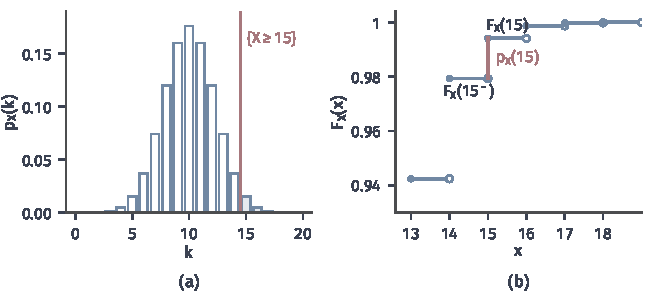
\includegraphics[width=112mm]{figures/07-probability/01-elementary-probability/matplotlib/tail-binomial-tail/figure.pdf}
 \caption{$X\sim\operatorname{Bin}(20,1/2)$的右尾。(a)质量表，浅蓝柱是事件$\{X\geq15\}$的质量，红线是阈值。(b)分布函数在$13$到$19$之间的阶梯，实心点是取到的值，空心点是左极限；红色竖线是$15$处的跳跃，高度为$p_X(15)$。}
 \label{fig:tail-binomial-tail}
\end{BookInlineFigure}

\paragraph{有密度的情形}
若$X$有密度$f_X$，单点概率为零，两种右尾相等，都等于密度在$t$右侧的面积：
\begin{equation}
 \mathbb{P}(X\geq t)=\mathbb{P}(X>t)=\int_t^{\infty}f_X(x)\,\mathrm{d}x .
 \label{eq:tail-density}
\end{equation}
三个模型足以展示尾部的不同衰减方式。$X\sim\operatorname{Exp}(1)$时积分得$\mathbb{P}(X>t)=\mathrm{e}^{-t}$，$t\geq0$。$Z\sim\mathcal{N}(0,1)$时右尾记作
\[
 Q(t)=\mathbb{P}(Z>t)=\int_t^{\infty}\frac{1}{\sqrt{2\pi}}\mathrm{e}^{-x^2/2}\,\mathrm{d}x ,
\]
它没有初等原函数，需要数值积分。常用的几个值是
\[
 Q(1)\approx0.1587,\quad Q(2)\approx0.02275,\quad Q(3)\approx0.00135 .
\]

第三个模型的尾部只按幂次衰减。对$\alpha>0$，在$[1,\infty)$上取密度$f_X(x)=\alpha x^{-\alpha-1}$，积分得
\begin{equation}
 \mathbb{P}(X>t)=\int_t^{\infty}\alpha x^{-\alpha-1}\,\mathrm{d}x=t^{-\alpha},\qquad t\geq1 .
 \label{eq:tail-pareto}
\end{equation}
令$t=1$得总质量为一，所以这确是密度。这个分布称为参数为$\alpha$的\term{Pareto分布}（Pareto distribution），$t<1$时$\mathbb{P}(X>t)=1$。本章用$\alpha=3$作为尾部较重的代表。

图~\ref{fig:tail-decay-shapes}把三条生存函数画在对数纵轴上。指数分布是一条直线，斜率为$-1$；高斯尾部向下弯，越来越陡，因为指数里是$t^2$；Pareto尾部越来越平，在$t=5$处仍有$0.008$，同一处高斯尾部已不到$3\times10^{-7}$。对数坐标把“远处还剩多少质量”的差别放大到了肉眼可见的程度。

\begin{BookInlineFigure}
 \centering
 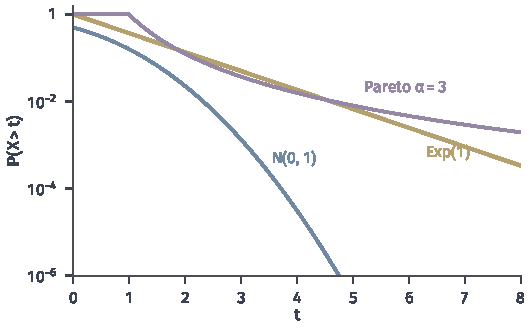
\includegraphics[width=90mm]{figures/07-probability/01-elementary-probability/matplotlib/tail-decay-shapes/figure.pdf}
 \caption{三种右尾，纵轴为对数刻度。蓝线为$\mathcal{N}(0,1)$的$Q(t)$，黄线为$\operatorname{Exp}(1)$的$\mathrm{e}^{-t}$，紫线为$\alpha=3$的Pareto分布的$\min\{1,t^{-3}\}$。}
 \label{fig:tail-decay-shapes}
\end{BookInlineFigure}

\paragraph{偏离中心的双侧事件}
很多时候关心的不是越过某个阈值，而是离某个中心$a$太远，例如测量值偏离真值至少$t$。对$t>0$，事件$\{\lvert X-a\rvert\geq t\}$拆成两个不相交的单侧事件：
\[
 \{\lvert X-a\rvert\geq t\}=\{X\geq a+t\}\cup\{X\leq a-t\} .
\]
两部分不相交，因为$a+t>a-t$。由加法规则和式~\eqref{eq:tail-closed}，
\begin{equation}
 \mathbb{P}(\lvert X-a\rvert\geq t)=1-F_X\bigl((a+t)^-\bigr)+F_X(a-t) .
 \label{eq:tail-two-sided}
\end{equation}
若$X$关于$a$对称，两部分相等，双侧概率是单侧的两倍。贯穿例子关于$10$对称，所以
\[
 \mathbb{P}(\lvert X-10\rvert\geq5)=2\,\mathbb{P}(X\geq15)=\frac{43400}{2^{20}}\approx0.04139 .
\]

分布不对称时两侧必须分开算。取$X\sim\operatorname{Exp}(1)$，均值为$1$，问偏离均值至少$t=0.5$的概率。左侧是$\{X\leq0.5\}$，右侧是$\{X\geq1.5\}$，分别为
\[
 \mathbb{P}(X\leq0.5)=1-\mathrm{e}^{-0.5}\approx0.3935,\qquad \mathbb{P}(X\geq1.5)=\mathrm{e}^{-1.5}\approx0.2231 .
\]
相加得$0.6166$，左侧贡献更大，见图~\ref{fig:tail-two-sided}。若$t\geq1$，左侧事件$\{X\leq1-t\}$要求$X\leq0$，概率为零，只剩右侧$\mathrm{e}^{-(1+t)}$。

\begin{BookInlineFigure}
 \centering
 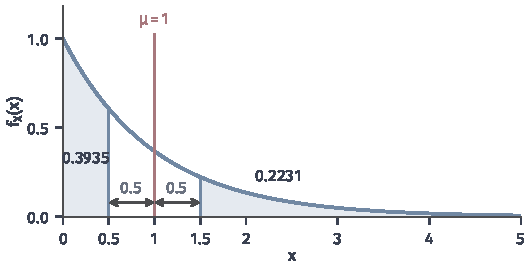
\includegraphics[width=90mm]{figures/07-probability/01-elementary-probability/matplotlib/tail-two-sided/figure.pdf}
 \caption{$X\sim\operatorname{Exp}(1)$偏离均值$\mu=1$至少$0.5$的事件。蓝线为密度，两块浅蓝区域是$\{X\leq0.5\}$与$\{X\geq1.5\}$，数字是各自的面积；红线标出均值。}
 \label{fig:tail-two-sided}
\end{BookInlineFigure}

\paragraph{尾概率与期望}
尾概率与期望之间有一条直接的联系。对非负整数值的变量，把$k\,p_X(k)$写成$k$个$p_X(k)$之和，再按“至少为$j$”重新归组：
\[
 \mathbb{E}[X]=\sum_{k\geq1}\sum_{j=1}^{k}p_X(k)=\sum_{j\geq1}\sum_{k\geq j}p_X(k)=\sum_{j\geq1}\mathbb{P}(X\geq j) .
\]
所有项非负，二重级数可以交换求和次序。对贯穿例子，把$\mathbb{P}(X\geq j)$对$j=1,\dots,20$相加，正好得到$10$。

有密度时，求和换成积分，并可以推广到$X$的函数。下面的\term{尾积分公式}说明期望完全由生存函数决定，后面检查矩与指数矩是否存在时要用它。

\begin{lemma}[尾积分公式]
\label{lem:tail-integral}
设$X\geq0$有密度$f_X$，$g$在$[0,\infty)$上连续可微且不减。则
\begin{equation}
 \mathbb{E}[g(X)]=g(0)+\int_0^{\infty}g'(s)\,\mathbb{P}(X>s)\,\mathrm{d}s ,
 \label{eq:tail-integral}
\end{equation}
两边同时有限或同时为$+\infty$。特别地，取$g(x)=x$与$g(x)=x^p$（$p>0$）得
\begin{equation}
 \mathbb{E}[X]=\int_0^{\infty}\mathbb{P}(X>s)\,\mathrm{d}s,\qquad \mathbb{E}[X^p]=\int_0^{\infty}p\,s^{p-1}\,\mathbb{P}(X>s)\,\mathrm{d}s .
 \label{eq:tail-integral-moments}
\end{equation}
\end{lemma}

\begin{proof}
由微积分基本定理，$g(x)-g(0)=\int_0^xg'(s)\,\mathrm{d}s$。两边乘$f_X(x)$并对$x\geq0$积分，得到
\[
 \mathbb{E}[g(X)]-g(0)=\int_0^{\infty}\Bigl(\int_0^{x}g'(s)\,\mathrm{d}s\Bigr)f_X(x)\,\mathrm{d}x .
\]
被积函数$g'(s)f_X(x)$在区域$0\leq s\leq x$上非负，所以可以交换积分次序，结果有限与否不受影响。交换的依据是非负函数的累次积分定理，可参考\BookChapterRef{chap:integration}{卷四第6章“积分”}；第~\ref{chap:probability-spaces}章会把它统一到概率的语言里。交换后内层对$x$从$s$积到$\infty$：
\[
 \mathbb{E}[g(X)]-g(0)=\int_0^{\infty}g'(s)\Bigl(\int_s^{\infty}f_X(x)\,\mathrm{d}x\Bigr)\mathrm{d}s .
\]
内层积分就是$\mathbb{P}(X>s)$，于是得到式~\eqref{eq:tail-integral}。
\end{proof}

用Pareto分布检验这个公式。$\alpha=3$时生存函数在$[0,1)$上为$1$，在$[1,\infty)$上为$s^{-3}$。代入式~\eqref{eq:tail-integral-moments}的第二式，对$0<p<3$，
\[
 \mathbb{E}[X^p]=\int_0^1p\,s^{p-1}\,\mathrm{d}s+\int_1^{\infty}p\,s^{p-4}\,\mathrm{d}s=1+\frac{p}{3-p}=\frac{3}{3-p} .
\]
$p=1$时得均值$3/2$，$p=2$时得$\mathbb{E}[X^2]=3$。若$p\geq3$，第二个积分发散，$p$阶矩为$+\infty$。尾部$s^{-3}$的衰减速度直接决定了哪些矩存在。

\paragraph{计算与估计}
已知完整分布时，尾概率是一个确定的数，按式~\eqref{eq:tail-closed}或式~\eqref{eq:tail-density}算出即可。反过来给定尾概率的水平去找阈值，就是第~\ref{chap:random-variables}章的分位数。直接计算的困难在于信息：很多时候只知道均值、方差之类的少数数值，或者完整分布虽然存在，却写不出可以求和、积分的形式。

这时能做的是给出\emph{上界}：找一个只依赖已知数值的量，保证所有具有这些数值的分布，其尾概率都不超过它。上界是一种保证，不是估计值；它必须对已知信息允许的最坏分布也成立。下面几节依次增加已知信息，看保证能收紧到什么程度。


\section{Markov不等式}
\label{sec:tail-markov}

回到响应时间。设$X\geq0$，平均$\mathbb{E}[X]=2$秒。有没有可能一半的请求都超过$5$秒？不可能：这一半请求单是自己就给平均值贡献了至少$0.5\times5=2.5$秒，已经超过$2$。这个“远处的质量至少按阈值计入平均”的想法，就是本节的全部内容。

\paragraph{重心的论证}
把分布看成数轴上总量为一的质量，期望是它的重心。质量全在$[0,\infty)$上时，落在$t$右边的那部分质量对重心的贡献至少是“质量乘$t$”；其余质量的贡献至少是$0$。重心又只有$\mathbb{E}[X]$那么远，所以远处的质量不能太多。

\begin{theorem}[Markov不等式]
\label{thm:tail-markov}
设随机变量$X\geq0$，$\mathbb{E}[X]<\infty$。则对每个$t>0$，
\begin{equation}
 \mathbb{P}(X\geq t)\leq\frac{\mathbb{E}[X]}{t} .
 \label{eq:tail-markov}
\end{equation}
\end{theorem}

这个结论称为\term{Markov不等式}（Markov inequality）。证明把“至少贡献$t$”写成两个随机变量之间的比较。

\begin{proof}
考虑示性变量$\mathbf{1}_{\{X\geq t\}}$，它在$X\geq t$时取$1$，否则取$0$。逐个样本点比较$t\,\mathbf{1}_{\{X\geq t\}}$与$X$：若$X\geq t$，左边是$t$，不超过$X$；若$X<t$，左边是$0$，由$X\geq0$也不超过$X$。所以
\[
 t\,\mathbf{1}_{\{X\geq t\}}\leq X .
\]
两边取期望。由期望的保序性和线性性（第~\ref{chap:random-variable-moments}章），以及示性变量的期望就是事件的概率，得到
\[
 t\,\mathbb{P}(X\geq t)\leq\mathbb{E}[X] .
\]
除以$t>0$即得式~\eqref{eq:tail-markov}。
\end{proof}

证明的关键一步是用一个函数从上方压住尾事件的示性函数。图~\ref{fig:tail-dominating}(a)画的就是这一点：蓝色台阶是$\mathbf{1}_{\{x\geq t\}}$，紫色直线是$x/t$，在$x\geq0$上直线处处不低于台阶。取期望后，台阶给出概率，直线给出$\mathbb{E}[X]/t$。另外两个子图是后两节要用的压法，换一个压住台阶的函数，就换一个不等式。

\begin{BookInlineFigure}
 \centering
 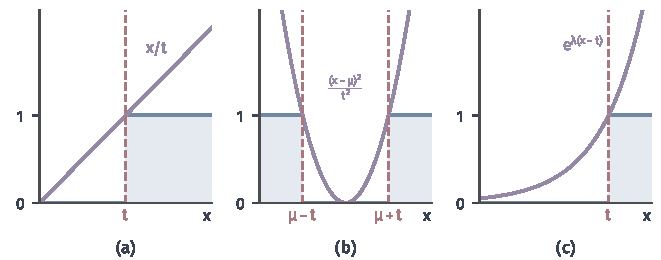
\includegraphics[width=112mm]{figures/07-probability/01-elementary-probability/matplotlib/tail-dominating/figure.pdf}
 \caption{用函数从上方压住尾事件的示性函数。蓝色台阶与浅蓝区域是示性函数，紫线是压住它的函数，红色虚线是阈值。(a)$x\geq0$上的$x/t$。(b)$(x-\mu)^2/t^2$。(c)$\mathrm{e}^{\lambda(x-t)}$，$\lambda>0$。}
 \label{fig:tail-dominating}
\end{BookInlineFigure}

\paragraph{搬动质量的图景}
同一个证明还可以看成搬动质量。把$[0,t)$里的质量全部搬到$0$，把$[t,\infty)$里的质量全部搬到$t$。每块质量只向左移动，重心只会左移；搬完以后，$t$处的质量仍是$\mathbb{P}(X\geq t)$，新重心是$t\,\mathbb{P}(X\geq t)$。于是新重心不超过原重心，这正是$t\,\mathbb{P}(X\geq t)\leq\mathbb{E}[X]$。

图~\ref{fig:tail-markov-mass}用一个六点分布演示。上排质量依次为$0.15$、$0.25$、$0.20$、$0.15$、$0.15$、$0.10$，位于$1$、$2$、$3$、$4$、$6$、$8$，重心为
\[
 \mu=0.15+0.5+0.6+0.6+0.9+0.8=3.55 .
\]
取$t=5$，右边有质量$0.25$。搬动后下排只剩$0$处的$0.75$和$5$处的$0.25$，重心变为$5\times0.25=1.25\leq3.55$。

\begin{BookInlineFigure}
 \centering
 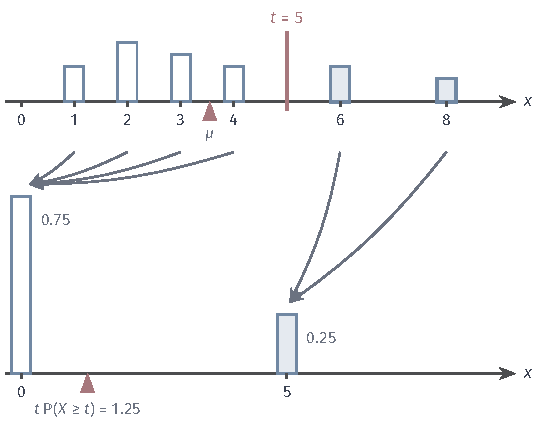
\includegraphics[width=92mm]{figures/07-probability/01-elementary-probability/tikz/tail-markov-mass/figure.pdf}
 \caption{Markov不等式的搬动质量论证。上排是原分布，浅蓝柱是$\{X\geq5\}$的质量，红线是阈值$t=5$，红三角是重心$\mu=3.55$。灰色箭头把$t$左边的质量搬到$0$，把右边的质量搬到$t$。下排是搬动后的两点分布，重心降为$t\,\mathbb{P}(X\geq t)=1.25$。}
 \label{fig:tail-markov-mass}
\end{BookInlineFigure}

\paragraph{面积的图景}
第三种看法用尾积分公式。由式~\eqref{eq:tail-integral-moments}，$\mathbb{E}[X]$是生存函数$s\mapsto\mathbb{P}(X>s)$下方的面积。对$0\leq s<t$，有$\{X\geq t\}\subseteq\{X>s\}$，所以生存函数在$[0,t)$上不低于$\mathbb{P}(X\geq t)$。宽为$t$、高为$\mathbb{P}(X\geq t)$的矩形整个落在曲线下方，面积不超过总面积。

图~\ref{fig:tail-layer-cake}取$X\sim\operatorname{Exp}(1)$与$t=2$。曲线下总面积是$\mu=1$，黄色矩形面积是$2\mathrm{e}^{-2}\approx0.271$。矩形之外的面积就是Markov不等式没有用上的部分：$t$左边曲线高出矩形的那一块，以及$t$右边的整个尾巴。

\begin{BookInlineFigure}
 \centering
 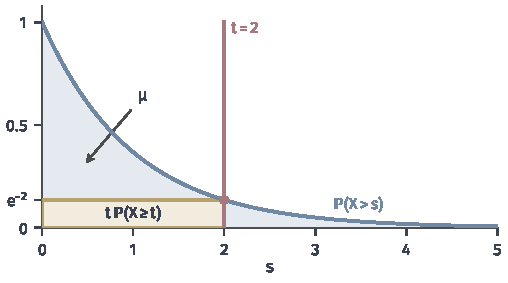
\includegraphics[width=86mm]{figures/07-probability/01-elementary-probability/matplotlib/tail-layer-cake/figure.pdf}
 \caption{$X\sim\operatorname{Exp}(1)$的生存函数（蓝线）。浅蓝区域面积等于$\mu=\mathbb{E}[X]=1$；黄色矩形宽$t=2$、高$\mathbb{P}(X\geq2)=\mathrm{e}^{-2}$，落在曲线下方，所以$t\,\mathbb{P}(X\geq t)\leq\mu$。}
 \label{fig:tail-layer-cake}
\end{BookInlineFigure}

\paragraph{条件的作用}
定理有三个条件，每一个都不能随便去掉。

第一是$X\geq0$。若允许负值，正负质量可以互相抵消，均值不再约束远处的质量。设$X$以各$1/2$的概率取$-100$和$100$，则$\mathbb{E}[X]=0$，但$\mathbb{P}(X\geq1)=1/2$，而式~\eqref{eq:tail-markov}的右边是$0$。证明中失效的一步正是$X<t$时“$0\leq X$”。

第二是$\mathbb{E}[X]<\infty$。若期望为$+\infty$，不等式右边是$+\infty$，仍然成立但不提供任何信息。第三是$t>0$：$t\leq0$时$\{X\geq t\}$是必然事件，概率为$1$，也无需估计。

\paragraph{这个界不能再改进}
Markov不等式只用到均值。它会不会只是证明粗糙，换一种论证就能更紧？答案是否定的：在“非负、均值为$\mu$”这一信息下，它已经是最好的保证。

\begin{theorem}[Markov界的最优性]
\label{thm:tail-markov-sharp}
设$\mu>0$，$t>0$。在所有满足$X\geq0$、$\mathbb{E}[X]=\mu$的随机变量中，$\mathbb{P}(X\geq t)$的最大值为
\begin{equation}
 \sup\,\mathbb{P}(X\geq t)=\min\Bigl\{1,\frac{\mu}{t}\Bigr\} .
 \label{eq:tail-markov-sharp}
\end{equation}
\end{theorem}

\begin{proof}
由Markov不等式和概率不超过$1$，每个这样的$X$都满足$\mathbb{P}(X\geq t)\leq\min\{1,\mu/t\}$。只需构造达到它的分布。

若$\mu\leq t$，令$X$以概率$\mu/t$取$t$，以概率$1-\mu/t$取$0$。它非负，均值为$t\cdot\mu/t=\mu$，并且$\mathbb{P}(X\geq t)=\mu/t$。

若$\mu>t$，令$X$恒等于$\mu$。它的均值是$\mu$，并且$\mathbb{P}(X\geq t)=1$。
\end{proof}

两点分布正是搬动质量后的形状：质量只放在$0$和$t$两处，没有一点“浪费”在比$t$更远的地方，也没有放在$0$与$t$之间。任何具体分布只要在这两种方式上偏离两点分布，它的尾概率就严格小于$\mu/t$。

\paragraph{与精确值比较}
保证与具体模型的实际尾概率可以差得很远。贯穿例子中$\mathbb{E}[X]=10$，Markov不等式给出
\[
 \mathbb{P}(X\geq15)\leq\frac{10}{15}=\frac23\approx0.667 ,
\]
而精确值是$0.0207$，相差三十多倍。指数分布$X\sim\operatorname{Exp}(1)$的均值为$1$，Markov界是$1/t$，精确值是$\mathrm{e}^{-t}$：$t=5$时前者是$0.2$，后者是$0.0067$。

图~\ref{fig:tail-markov-compare}在对数纵轴上画出两组比较。精确尾部在两个例子中都下降得飞快，Markov界只按$1/t$缓慢下降。差距的来源并不是证明不精细，而是信息太少：界必须同时照顾到两点分布那样的极端情形。要得到更好的界，只能使用更多关于分布的信息。

\begin{BookInlineFigure}
 \centering
 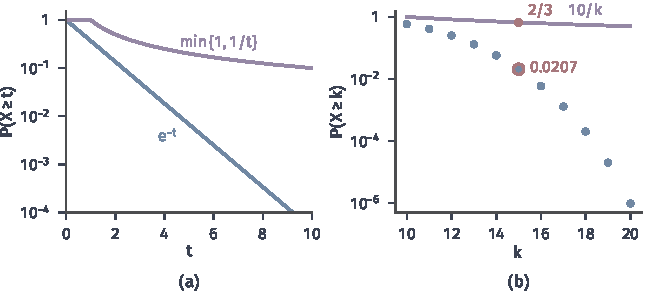
\includegraphics[width=112mm]{figures/07-probability/01-elementary-probability/matplotlib/tail-markov-compare/figure.pdf}
 \caption{Markov界（紫线）与精确尾概率（蓝色），纵轴为对数刻度。(a)$X\sim\operatorname{Exp}(1)$，精确值$\mathrm{e}^{-t}$。(b)$X\sim\operatorname{Bin}(20,1/2)$，蓝点为$\mathbb{P}(X\geq k)$，紫线为$10/k$，红色标出$k=15$处的$2/3$与$0.0207$。}
 \label{fig:tail-markov-compare}
\end{BookInlineFigure}

\paragraph{一般形式}
压住示性函数的不必是直线。只要函数$g$非负且不减，事件$\{X\geq t\}$就包含在$\{g(X)\geq g(t)\}$之中，对$g(X)$用Markov不等式即可。下面的形式是后面三节的共同出发点。

\begin{lemma}[Markov不等式的一般形式]
\label{lem:tail-markov-general}
设$g$是$\mathbb{R}$上的非负不减函数，$t$满足$g(t)>0$，且$\mathbb{E}[g(X)]<\infty$。则
\begin{equation}
 \mathbb{P}(X\geq t)\leq\frac{\mathbb{E}[g(X)]}{g(t)} .
 \label{eq:tail-markov-general}
\end{equation}
\end{lemma}

\begin{proof}
若$X\geq t$，由$g$不减得$g(X)\geq g(t)$，所以$\{X\geq t\}\subseteq\{g(X)\geq g(t)\}$，前者的概率不超过后者。$g(X)$非负，期望有限，$g(t)>0$，对它用定理~\ref{thm:tail-markov}：
\[
 \mathbb{P}(X\geq t)\leq\mathbb{P}\bigl(g(X)\geq g(t)\bigr)\leq\frac{\mathbb{E}[g(X)]}{g(t)} .
\]
这就是式~\eqref{eq:tail-markov-general}。
\end{proof}

这里不再要求$X\geq0$，非负性转移给了$g$。选择$g$就是选择要用分布的哪一项信息：对非负变量$\lvert X-a\rvert$取$g(s)=\max\{s,0\}^p$，用的是$p$阶绝对矩；对$X$本身取$g(x)=\mathrm{e}^{\lambda x}$，用的是指数矩。$g$在远处增长越快，远处的质量在$\mathbb{E}[g(X)]$里被放得越大，界就可能衰减得越快；代价是$\mathbb{E}[g(X)]$有限的要求越强。


\section{Chebyshev不等式}
\label{sec:tail-chebyshev}

测量值会偏高也会偏低，我们常关心的是它离均值有多远，而不是越过哪一个固定阈值。偏离$X-\mu$可正可负，Markov不等式不能直接用；取绝对值或平方以后才非负。平方的好处是它的期望正是方差，一个最常知道的数。

\paragraph{转动惯量的论证}
继续把分布看成质量。方差$\operatorname{Var}(X)=\mathbb{E}[(X-\mu)^2]$是质量绕重心$\mu$的转动惯量：每块质量按到重心距离的平方加权。离重心至少$t$的质量，对转动惯量的贡献至少是“质量乘$t^2$”。转动惯量只有$\sigma^2$那么大，所以远离重心的质量至多是$\sigma^2/t^2$。

\begin{theorem}[Chebyshev不等式]
\label{thm:tail-chebyshev}
设$X$的方差有限，记$\mu=\mathbb{E}[X]$，$\sigma^2=\operatorname{Var}(X)$。则对每个$t>0$，
\begin{equation}
 \mathbb{P}(\lvert X-\mu\rvert\geq t)\leq\frac{\sigma^2}{t^2} .
 \label{eq:tail-chebyshev}
\end{equation}
\end{theorem}

这个结论称为\term{Chebyshev不等式}（Chebyshev inequality）。

\begin{proof}
因为$t>0$，两个非负数$\lvert X-\mu\rvert$与$t$的大小关系在平方后保持不变，所以两个事件相同：
\[
 \{\lvert X-\mu\rvert\geq t\}=\{(X-\mu)^2\geq t^2\} .
\]
$(X-\mu)^2$是非负随机变量，期望为$\sigma^2<\infty$。对它在阈值$t^2>0$处用定理~\ref{thm:tail-markov}，得到
\[
 \mathbb{P}\bigl((X-\mu)^2\geq t^2\bigr)\leq\frac{\mathbb{E}[(X-\mu)^2]}{t^2}=\frac{\sigma^2}{t^2} .
\]
两个事件相同，这就是式~\eqref{eq:tail-chebyshev}。
\end{proof}

压住示性函数的函数这次是抛物线，见图~\ref{fig:tail-dominating}(b)：$(x-\mu)^2/t^2$在$\lvert x-\mu\rvert\geq t$时不小于$1$，在其他地方不小于$0$。与直线相比，抛物线在两侧同时向上，所以一次控制住两个方向的偏离。

\paragraph{以标准差为单位}
当$\sigma>0$时，取$t=k\sigma$，式~\eqref{eq:tail-chebyshev}成为
\begin{equation}
 \mathbb{P}(\lvert X-\mu\rvert\geq k\sigma)\leq\frac{1}{k^2},\qquad k>0 .
 \label{eq:tail-chebyshev-k}
\end{equation}
它对每个方差有限的分布都成立。取$k=2$和$k=3$，任何这样的分布至少有$75\%$的质量落在均值两侧两个标准差以内，至少有$1-1/9\approx88.9\%$落在三个标准差以内。$k\leq1$时右边不小于$1$，不提供信息。

\paragraph{条件的作用}
定理只要求方差有限，不要求非负，也不要求对称。方差无穷时右边是$+\infty$，不等式没有内容；第~\ref{chap:common-distributions}章中自由度$\nu\leq2$的t分布就是这样，这时只能改用阶数更低的矩，见下一节。式~\eqref{eq:tail-chebyshev}控制的是双侧事件。单侧事件$\{X\geq\mu+t\}$包含在其中，所以同一个界也适用于单侧，只是不一定紧。

\paragraph{这个界同样不能再改进}
与Markov不等式一样，只知道均值和方差时，$\sigma^2/t^2$已经是最好的保证。设$0<\sigma\leq t$，构造三点分布：
\[
 \mathbb{P}(X=\mu-t)=\mathbb{P}(X=\mu+t)=\frac{\sigma^2}{2t^2},\qquad \mathbb{P}(X=\mu)=1-\frac{\sigma^2}{t^2} .
\]
它关于$\mu$对称，所以均值为$\mu$。偏离为$\pm t$的两点各贡献$t^2\cdot\sigma^2/(2t^2)$，合起来方差为
\[
 \operatorname{Var}(X)=2\cdot t^2\cdot\frac{\sigma^2}{2t^2}=\sigma^2 ,
\]
而$\mathbb{P}(\lvert X-\mu\rvert\geq t)=\sigma^2/t^2$，等号成立。

这个分布的形状与Markov的两点分布同出一辙：远处的质量恰好放在距离$t$处，一点也不再往外放，其余质量全部堆在中心，不贡献转动惯量。图~\ref{fig:tail-chebyshev-extremal}取$\mu=0$，$\sigma=1$，$t=2$，三点的质量为$1/8,3/4,1/8$，双侧尾概率是$1/4$；同样均值和方差的标准高斯分布，双侧尾概率只有$0.0455$。

\begin{BookInlineFigure}
 \centering
 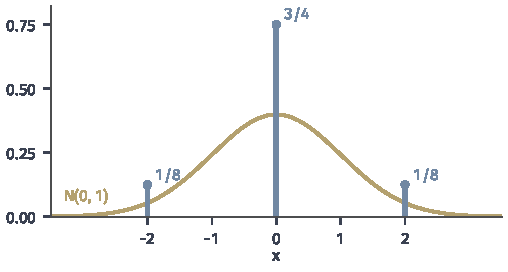
\includegraphics[width=86mm]{figures/07-probability/01-elementary-probability/matplotlib/tail-chebyshev-extremal/figure.pdf}
 \caption{使Chebyshev不等式取等号的三点分布（蓝色竖线，$\mu=0$，$\sigma=1$，$t=2$），质量$1/8,3/4,1/8$位于$-2,0,2$。黄线是均值、方差相同的$\mathcal{N}(0,1)$密度。}
 \label{fig:tail-chebyshev-extremal}
\end{BookInlineFigure}

\paragraph{与精确值比较}
由第~\ref{chap:common-distributions}章，贯穿例子的方差是$20\cdot\frac12\cdot\frac12=5$。取$t=5$，
\[
 \mathbb{P}(\lvert X-10\rvert\geq5)\leq\frac{5}{25}=0.2 .
\]
精确值是$0.0414$，界大了约五倍。单侧事件$\{X\geq15\}$也得到上界$0.2$，比Markov不等式的$2/3$好得多。改进来自两项新信息：方差告诉我们分布有多分散，均值作为中心使界只依赖偏离而不依赖原点的位置。

其他模型上可以看到同样的差距。对$Z\sim\mathcal{N}(0,1)$，
\[
 k=2:\ \tfrac14\ \text{对}\ 0.0455,\qquad k=3:\ \tfrac19\approx0.111\ \text{对}\ 0.0027 .
\]
对$X\sim\operatorname{Unif}(0,1)$，$\mu=1/2$，$\sigma^2=1/12$。$0<t\leq1/2$时精确值是$\mathbb{P}(\lvert X-1/2\rvert\geq t)=1-2t$。取$t=0.4$，精确值为$0.2$，界为$1/(12\times0.16)\approx0.521$。$t>1/2$时精确值是$0$，界却始终为正：Chebyshev不等式不知道分布的取值范围有界。

\paragraph{均值和方差不能决定尾部}
上面的比较说明，均值和方差相同的分布，尾部可以完全不同。图~\ref{fig:tail-same-variance}画出五个均值为$0$、方差为$1$的分布的双侧尾概率$\mathbb{P}(\lvert X\rvert\geq k)$：$[-\sqrt3,\sqrt3]$上的均匀分布，标准高斯分布，尺度为$1/\sqrt2$的Laplace分布，以及以各$1/2$概率取$\pm1$的两点分布。在$k=2$处，五个值分别是
\[
 0,\qquad 0.0455,\qquad \mathrm{e}^{-2\sqrt2}\approx0.0591,\qquad 0,\qquad \tfrac14 ,
\]
最后一个属于该处的三点极端分布。紫色曲线$1/k^2$是所有这些曲线的包络。

\begin{BookInlineFigure}
 \centering
 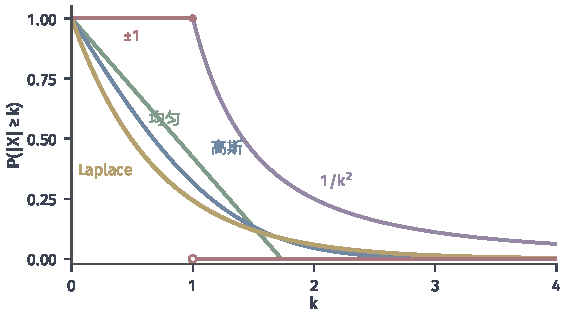
\includegraphics[width=96mm]{figures/07-probability/01-elementary-probability/matplotlib/tail-same-variance/figure.pdf}
 \caption{均值为$0$、方差为$1$的几个分布的双侧尾概率$\mathbb{P}(\lvert X\rvert\geq k)$。绿线为$[-\sqrt3,\sqrt3]$上的均匀分布，蓝线为$\mathcal{N}(0,1)$，黄线为尺度$1/\sqrt2$的Laplace分布，红线为取$\pm1$的两点分布，紫线为Chebyshev界$\min\{1,1/k^2\}$。}
 \label{fig:tail-same-variance}
\end{BookInlineFigure}

包络之下，曲线的形状由均值和方差之外的信息决定：均匀分布在$\sqrt3$处截断，两点分布在$1$处一下跳到零，Laplace分布的尾部比高斯分布更重。从$1/k^2$出发要把界进一步压低，就得知道分布在远处的更多情况，下一节用更高阶的矩来提供这样的信息。


\section{高阶矩上界}
\label{sec:tail-higher-moments}

Chebyshev不等式用平方给远处的质量加权。若把平方换成四次方、六次方，远处的质量在期望里被放得更大，同样大小的矩就迫使远处的质量更少。代价也很明显：要知道更高阶的矩，并且它要有限。

\paragraph{一般的矩上界}
设$a$是任意给定的中心，不必是均值。对非负变量$\lvert X-a\rvert$和$p>0$，函数$s\mapsto s^p$在$[0,\infty)$上严格增，所以对$t>0$，“偏离至少$t$”与“偏离的$p$次方至少$t^p$”是同一个事件。

\begin{theorem}[矩上界]
\label{thm:tail-moment}
设$p>0$，$a\in\mathbb{R}$，且$\mathbb{E}\lvert X-a\rvert^p<\infty$。则对每个$t>0$，
\begin{equation}
 \mathbb{P}(\lvert X-a\rvert\geq t)\leq\frac{\mathbb{E}\lvert X-a\rvert^p}{t^p} .
 \label{eq:tail-moment}
\end{equation}
\end{theorem}

\begin{proof}
因为$t>0$，$p>0$，幂函数$s\mapsto s^p$在$[0,\infty)$上严格增，所以$\lvert X-a\rvert\geq t$当且仅当$\lvert X-a\rvert^p\geq t^p$。$\lvert X-a\rvert^p$非负，期望有限，对它在阈值$t^p>0$处用定理~\ref{thm:tail-markov}：
\[
 \mathbb{P}(\lvert X-a\rvert\geq t)=\mathbb{P}\bigl(\lvert X-a\rvert^p\geq t^p\bigr)\leq\frac{\mathbb{E}\lvert X-a\rvert^p}{t^p} .
\]
这就是式~\eqref{eq:tail-moment}。
\end{proof}

式~\eqref{eq:tail-moment}称为\term{矩上界}（moment bound）。$p=2$、$a=\mu$时它就是Chebyshev不等式；$p=1$时它用的是平均绝对偏离；$p$也可以取非整数，例如$0<p<1$，这在均值都不存在时仍然可用。界按$t^{-p}$衰减，阶数越高，远处衰减越快。

\paragraph{存在条件随阶数加强}
由第~\ref{chap:random-variable-moments}章，$0<p<q$时，$q$阶绝对矩有限蕴含$p$阶绝对矩有限，反之不然。所以使用更高阶的矩是在假设更多。Pareto分布把这一点表现得很清楚：$\alpha=3$时，由第~\ref{sec:tail-events}节的计算，
\[
 \mathbb{E}[X^p]=\frac{3}{3-p},\qquad 0<p<3 ,
\]
$p\geq3$时为$+\infty$。阶数趋于$3$时矩本身趋于无穷，界$3/((3-p)t^p)$的系数随之变大。同样，自由度为$\nu$的t分布只有$p<\nu$阶的绝对矩有限。

\paragraph{贯穿例子的四阶与六阶矩}
对$X\sim\operatorname{Bin}(20,1/2)$，取中心$a=10$。由对称性，$p$阶中心绝对矩是
\[
 m_p=\mathbb{E}\lvert X-10\rvert^p=\frac{2}{2^{20}}\sum_{j=1}^{10}\binom{20}{10+j}j^p .
\]
用表~\ref{tab:tail-binomial}逐项相乘。$p=2$时十项之和是$2621440$，于是$m_2=5$，与方差一致。$p=4$时十项依次为
\[
 \begin{gathered}
 167960,\ 2015520,\ 6279120,\ 9922560,\ 9690000,\\
 6279120,\ 2737140,\ 778240,\ 131220,\ 10000,
 \end{gathered}
\]
和为$38010880$。$p=6$时同样相加，和为$887357440$。乘以$2/2^{20}$，得到
\[
 m_2=5,\qquad m_4=72.5,\qquad m_6=1692.5 .
\]

在$t=5$处比较三个界：
\[
 \frac{m_2}{5^2}=0.2,\qquad \frac{m_4}{5^4}=0.116,\qquad \frac{m_6}{5^6}\approx0.108 .
\]
阶数越高越接近精确值$0.0414$。但在$t=3$处情况相反：
\[
 \frac{m_2}{3^2}\approx0.556,\qquad \frac{m_4}{3^4}\approx0.895,\qquad \frac{m_6}{3^6}\approx2.32 .
\]
六阶的界大于$1$，毫无用处，二阶的界反而最好。

\paragraph{高阶不一定更紧}
原因在于矩把\emph{所有}偏离都按$p$次方加权。偏离小于$t$的质量在$\lvert x-a\rvert^p/t^p$中被压小，偏离大于$t$的质量被放大。$t$较小时，大量质量的偏离与$t$相当或更大，高阶矩被它们放大得很厉害；$t$较大时，远处的质量很少，高阶矩被放大的部分有限，而$t^p$增长得更快。

两个界的交点可以直接解出。四阶界小于二阶界，当且仅当$m_4/t^4<m_2/t^2$，即
\[
 t^2>\frac{m_4}{m_2}=\frac{72.5}{5}=14.5,\qquad t>3.81 .
\]
同理，六阶界小于四阶界当且仅当$t^2>m_6/m_4\approx23.3$，即$t>4.83$。图~\ref{fig:tail-binomial-moment-bounds}显示了这种依次接替：每一阶的界在某个阈值以后才成为最好的。

\begin{BookInlineFigure}
 \centering
 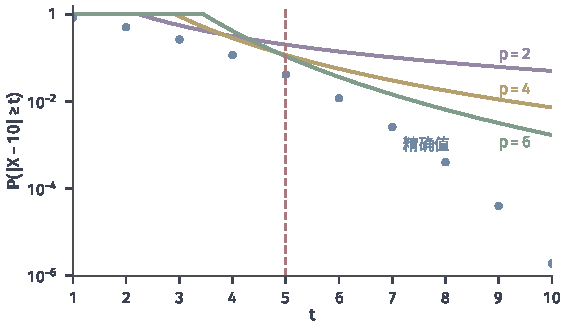
\includegraphics[width=96mm]{figures/07-probability/01-elementary-probability/matplotlib/tail-binomial-moment-bounds/figure.pdf}
 \caption{$X\sim\operatorname{Bin}(20,1/2)$的双侧尾概率$\mathbb{P}(\lvert X-10\rvert\geq t)$（蓝点）与矩上界$\min\{1,m_p/t^p\}$：紫线$p=2$，黄线$p=4$，绿线$p=6$。纵轴为对数刻度，红色虚线标出$t=5$。}
 \label{fig:tail-binomial-moment-bounds}
\end{BookInlineFigure}

\paragraph{给定阈值时选择阶数}
既然没有一个阶数处处最好，自然的做法是对给定的$t$，在所有可用的阶数中取最小的界。标准高斯分布的各阶矩都有限，可以把这件事算到底。记$\varphi(x)=\mathrm{e}^{-x^2/2}/\sqrt{2\pi}$，它满足$\varphi'(x)=-x\varphi(x)$。对$p\geq0$分部积分，边界项因$\varphi$衰减极快而为零，得到
\[
 \mathbb{E}[Z^{p+2}]=\int_{-\infty}^{\infty}x^{p+1}\cdot x\varphi(x)\,\mathrm{d}x=(p+1)\int_{-\infty}^{\infty}x^{p}\varphi(x)\,\mathrm{d}x=(p+1)\,\mathbb{E}[Z^p] .
\]
从$\mathbb{E}[Z^0]=1$出发，偶数阶矩为
\[
 \mathbb{E}[Z^{p}]=(p-1)(p-3)\cdots3\cdot1,\qquad p=2,4,6,\dots .
\]因此从$p$阶换到$p+2$阶，界乘上因子
\[
 \frac{\mathbb{E}[Z^{p+2}]/t^{p+2}}{\mathbb{E}[Z^p]/t^p}=\frac{p+1}{t^2} .
\]
只要$p+1<t^2$，提高阶数就让界变小；一旦$p+1>t^2$，再提高就变大。

$t=2$时$t^2=4$，从$p=2$到$p=4$乘$3/4$，再到$p=6$乘$5/4$，所以最好的偶数阶是$p=4$，界为$3/16=0.1875$。$t=3$时$t^2=9$，从$p=6$到$p=8$乘$7/9$，从$p=8$到$p=10$乘$9/9=1$，界在$p=8$和$p=10$处同为
\[
 \frac{\mathbb{E}[Z^8]}{3^8}=\frac{105}{6561}\approx0.0160 .
\]
奇数阶的绝对矩也可以计算，$p=9$时略小，约为$0.0156$；精确值是$2Q(3)\approx0.0027$。

图~\ref{fig:tail-normal-moment-order}把界作为阶数的函数画出来：曲线先降后升，最低点随$t$右移。最优阶数大约是$t^2$，阈值越远，越要用高阶矩。若只允许用某个固定阶数$p$，界只能按$t^{-p}$衰减，而高斯尾部比任何幂次都衰减得快。要跟上这种衰减，就需要把各阶矩一起利用，这正是下一节指数矩的作用。

\begin{BookInlineFigure}
 \centering
 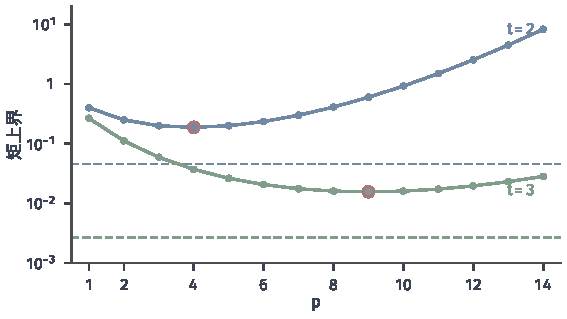
\includegraphics[width=96mm]{figures/07-probability/01-elementary-probability/matplotlib/tail-normal-moment-order/figure.pdf}
 \caption{$Z\sim\mathcal{N}(0,1)$的矩上界$\mathbb{E}\lvert Z\rvert^p/t^p$随阶数$p$的变化，纵轴为对数刻度。蓝色为$t=2$，绿色为$t=3$，红圈是整数阶中的最小值，同色虚线是精确值$\mathbb{P}(\lvert Z\rvert\geq t)$。}
 \label{fig:tail-normal-moment-order}
\end{BookInlineFigure}


\section{指数矩上界}
\label{sec:tail-exponential-moments}

上一节看到，对高斯分布，阈值越远就要用越高阶的矩，而每次都要在许多阶之间挑选。能否一次把所有阶的矩都用上？指数函数的幂级数
\[
 \mathrm{e}^{\lambda x}=\sum_{k\geq0}\frac{\lambda^kx^k}{k!}
\]
恰好把各阶幂次按权重$\lambda^k/k!$加在一起。用$\mathrm{e}^{\lambda x}$去压尾事件的示性函数，得到的界只依赖一个期望。

\paragraph{矩母函数}
先给这个期望一个名字。它对有些$\lambda$有限，对有些$\lambda$可能是$+\infty$，所以同时记录它在哪里有限。

\begin{definition}[矩母函数]
\label{def:tail-mgf}
随机变量$X$的\term{矩母函数}（moment generating function）是
\begin{equation}
 M_X(\lambda)=\mathbb{E}\bigl[\mathrm{e}^{\lambda X}\bigr],\qquad \lambda\in\mathbb{R},
 \label{eq:tail-mgf}
\end{equation}
其中$\mathrm{e}^{\lambda X}>0$，期望总有定义，取值在$(0,+\infty]$中。
\end{definition}

总有$M_X(0)=1$。若$M_X(\lambda)$在$0$附近有限，把$\mathrm{e}^{\lambda X}$按幂级数展开并逐项取期望，$\lambda^k$的系数正是$\mathbb{E}[X^k]/k!$，这就是“矩母”这个名字的来历。逐项取期望的合理性以及矩母函数怎样识别分布，在第~\ref{chap:weak-convergence-of-distributions}章讨论；本节只把$M_X(\lambda)$当作一个可以计算的期望来用。

\paragraph{指数矩上界}
函数$x\mapsto\mathrm{e}^{\lambda x}$在$\lambda>0$时正且严格增，满足引理~\ref{lem:tail-markov-general}的全部条件，并且不要求$X$非负。

\begin{theorem}[指数矩上界]
\label{thm:tail-chernoff}
设$\lambda>0$，$M_X(\lambda)<\infty$。则对每个$t\in\mathbb{R}$，
\begin{equation}
 \mathbb{P}(X\geq t)\leq\mathrm{e}^{-\lambda t}M_X(\lambda) .
 \label{eq:tail-chernoff-lambda}
\end{equation}
因而
\begin{equation}
 \mathbb{P}(X\geq t)\leq\inf_{\lambda>0}\mathrm{e}^{-\lambda t}M_X(\lambda) ,
 \label{eq:tail-chernoff}
\end{equation}
其中$M_X(\lambda)=+\infty$的$\lambda$不起作用。
\end{theorem}

\begin{proof}
在引理~\ref{lem:tail-markov-general}中取$g(x)=\mathrm{e}^{\lambda x}$。它非负、不减，$g(t)=\mathrm{e}^{\lambda t}>0$，$\mathbb{E}[g(X)]=M_X(\lambda)<\infty$，所以
\[
 \mathbb{P}(X\geq t)\leq\frac{M_X(\lambda)}{\mathrm{e}^{\lambda t}}=\mathrm{e}^{-\lambda t}M_X(\lambda) .
\]
左边不依赖$\lambda$，对所有使右边有限的$\lambda>0$取下确界，得到式~\eqref{eq:tail-chernoff}。
\end{proof}

式~\eqref{eq:tail-chernoff}称为\term{Chernoff界}（Chernoff bound）。图~\ref{fig:tail-dominating}(c)是它的压法：$\mathrm{e}^{\lambda(x-t)}$在$x\geq t$时不小于$1$，在$x<t$时为正。$\lambda$控制这条曲线的形状：$\lambda$大时曲线在$t$左边迅速趋于零，把近处的质量压得很小，但在$t$右边陡峭上升，把远处的质量放得很大；$\lambda$小时正好相反。最优的$\lambda$在两者之间折中。

取对数可以把式~\eqref{eq:tail-chernoff}写成指数形式。记$\psi_X(\lambda)=\ln M_X(\lambda)$，则
\begin{equation}
 \mathbb{P}(X\geq t)\leq\exp\Bigl(-\sup_{\lambda>0}\bigl(\lambda t-\psi_X(\lambda)\bigr)\Bigr) .
 \label{eq:tail-chernoff-exponent}
\end{equation}
在下面的例子中，$\lambda t-\psi_X(\lambda)$都可以求导找到最大点。

\paragraph{高斯分布}
先计算$Z\sim\mathcal{N}(0,1)$的矩母函数。把指数部分配方，$\lambda x-x^2/2=\lambda^2/2-(x-\lambda)^2/2$，于是
\[
 M_Z(\lambda)=\mathrm{e}^{\lambda^2/2}\int_{-\infty}^{\infty}\frac{1}{\sqrt{2\pi}}\mathrm{e}^{-(x-\lambda)^2/2}\,\mathrm{d}x=\mathrm{e}^{\lambda^2/2} .
\]
最后的积分是平移后的高斯密度，等于$1$。它对一切实数$\lambda$有限。

代入式~\eqref{eq:tail-chernoff-lambda}，对$t>0$，
\[
 \mathbb{P}(Z\geq t)\leq\mathrm{e}^{-\lambda t+\lambda^2/2} .
\]
指数$-\lambda t+\lambda^2/2$是$\lambda$的二次函数，在$\lambda=t$处取最小值$-t^2/2$。所以
\begin{equation}
 \mathbb{P}(Z\geq t)\leq\mathrm{e}^{-t^2/2},\qquad t>0 .
 \label{eq:tail-gauss-chernoff}
\end{equation}
对$X\sim\mathcal{N}(\mu,\sigma^2)$，写$X=\mu+\sigma Z$，事件$\{X-\mu\geq t\}$就是$\{Z\geq t/\sigma\}$，得到
\[
 \mathbb{P}(X-\mu\geq t)\leq\mathrm{e}^{-t^2/(2\sigma^2)},\qquad t>0 .
\]

图~\ref{fig:tail-chernoff-lambda}(b)画出$t=1,2,3$时的函数$\lambda\mapsto\mathrm{e}^{-\lambda t+\lambda^2/2}$，红点是最小点$\lambda=t$。三个最小值与精确值的对比是
\[
 \begin{gathered}
 t=1:\ 0.607\ \text{对}\ 0.1587,\qquad t=2:\ 0.135\ \text{对}\ 0.0228,\\
 t=3:\ 0.0111\ \text{对}\ 0.00135 .
 \end{gathered}
\]
精确值与上界之比依次约为$0.26$、$0.17$、$0.12$，变化缓慢；起主导作用的因子$\mathrm{e}^{-t^2/2}$被界完整地抓住了。与之相比，Chebyshev界$1/t^2$在$t=3$处是$0.111$，大了八十多倍。

\paragraph{贯穿例子}
对$X\sim\operatorname{Bin}(20,1/2)$，按定义求和并用二项式定理：
\[
 M_X(\lambda)=\sum_{k=0}^{20}\binom{20}{k}2^{-20}\mathrm{e}^{\lambda k}=\Bigl(\frac{1+\mathrm{e}^{\lambda}}{2}\Bigr)^{20} .
\]
在$t=15$处，要最小化的函数是
\[
 h(\lambda)=\ln\bigl(\mathrm{e}^{-15\lambda}M_X(\lambda)\bigr)=-15\lambda+20\ln(1+\mathrm{e}^{\lambda})-20\ln2 .
\]

对$\lambda$求导并令导数为零：
\[
 h'(\lambda)=-15+\frac{20\,\mathrm{e}^{\lambda}}{1+\mathrm{e}^{\lambda}}=0 .
\]
由$4\mathrm{e}^{\lambda}=3(1+\mathrm{e}^{\lambda})$解得
\[
 \mathrm{e}^{\lambda}=3,\qquad \lambda=\ln3\approx1.099 .
\]
再求一次导数，
\[
 h''(\lambda)=\frac{20\,\mathrm{e}^{\lambda}}{(1+\mathrm{e}^{\lambda})^2}>0 ,
\]
所以$h'$严格增，$\lambda=\ln3$是唯一的最小点。

代回去，$M_X(\ln3)=2^{20}$，$\mathrm{e}^{-15\ln3}=3^{-15}$，所以
\begin{equation}
 \mathbb{P}(X\geq15)\leq\frac{2^{20}}{3^{15}}=\frac{1048576}{14348907}\approx0.0731 .
 \label{eq:tail-binomial-chernoff}
\end{equation}
这比六阶矩界$0.108$更好，距精确值$0.0207$只差约$3.5$倍。图~\ref{fig:tail-chernoff-lambda}(a)显示了$\lambda$的选择：$\lambda$太小，指数函数几乎是常数，界接近$1$；$\lambda$太大，远处的质量被放得过大，界又上升。

\begin{BookInlineFigure}
 \centering
 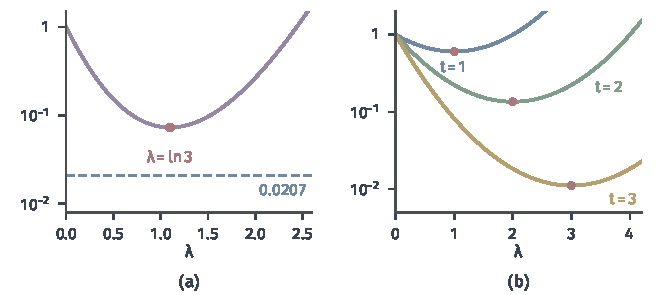
\includegraphics[width=112mm]{figures/07-probability/01-elementary-probability/matplotlib/tail-chernoff-lambda/figure.pdf}
 \caption{指数矩上界作为$\lambda$的函数，纵轴为对数刻度，红点为最小点。(a)$X\sim\operatorname{Bin}(20,1/2)$，$t=15$，紫线为$\mathrm{e}^{-15\lambda}M_X(\lambda)$，最小值$2^{20}/3^{15}\approx0.0731$在$\lambda=\ln3$处取到，蓝色虚线为精确值$0.0207$。(b)$Z\sim\mathcal{N}(0,1)$，$t=1,2,3$时的$\mathrm{e}^{-\lambda t+\lambda^2/2}$，最小点为$\lambda=t$。}
 \label{fig:tail-chernoff-lambda}
\end{BookInlineFigure}

同样的计算适用于一般的二项分布。设$X\sim\operatorname{Bin}(n,p)$，$0<p<1$，阈值写成$na$，$p<a<1$。$M_X(\lambda)=(1-p+p\mathrm{e}^{\lambda})^n$，令导数为零得$\mathrm{e}^{\lambda}=a(1-p)/\bigl(p(1-a)\bigr)$，它大于$1$，所以$\lambda>0$。代回整理，得到
\begin{equation}
 \mathbb{P}(X\geq na)\leq\Bigl[\Bigl(\frac{p}{a}\Bigr)^{a}\Bigl(\frac{1-p}{1-a}\Bigr)^{1-a}\Bigr]^{n} .
 \label{eq:tail-binomial-chernoff-general}
\end{equation}
方括号里的数小于$1$。比例$a$固定时，界随试验次数$n$按几何级数缩小。取$n=20$，$p=1/2$，$a=3/4$，方括号里是$(2/3)^{3/4}2^{1/4}\approx0.8774$，其$20$次方回到$0.0731$。

\paragraph{指数分布}
对$X\sim\operatorname{Exp}(1)$，矩母函数是
\[
 M_X(\lambda)=\int_0^{\infty}\mathrm{e}^{\lambda x}\mathrm{e}^{-x}\,\mathrm{d}x=\begin{cases}\dfrac{1}{1-\lambda}, & \lambda<1,\\ +\infty, & \lambda\geq1 .\end{cases}
\]
$\lambda\geq1$时被积函数不趋于零，积分发散。所以下确界只能在$0<\lambda<1$中取。

对$t>1$，取对数后要最小化的是
\[
 \ln\frac{\mathrm{e}^{-\lambda t}}{1-\lambda}=-\lambda t-\ln(1-\lambda),\qquad 0<\lambda<1 .
\]
它的导数为$-t+1/(1-\lambda)$，零点是$\lambda=1-1/t\in(0,1)$，导数在它左边为负、右边为正。代回得
\begin{equation}
 \mathbb{P}(X\geq t)\leq t\,\mathrm{e}^{1-t},\qquad t>1 .
 \label{eq:tail-exp-chernoff}
\end{equation}
$t\leq1$时导数在$(0,1)$上处处非负，下确界在$\lambda\to0$时取到，界为$1$。

精确值是$\mathrm{e}^{-t}$，两者之比为$\mathrm{e}\,t$：$t=5$时界为$0.0916$，精确值为$0.0067$。指数衰减率$\mathrm{e}^{-t}$被保留了，丢掉的是一个线性因子。原因是$\lambda$不能取到$1$：要完全抓住$\mathrm{e}^{-t}$，需要$\lambda=1$，而那里矩母函数已经是无穷。图~\ref{fig:tail-chernoff-compare}把两个模型上的指数矩上界与较弱的界放在一起。

\begin{BookInlineFigure}
 \centering
 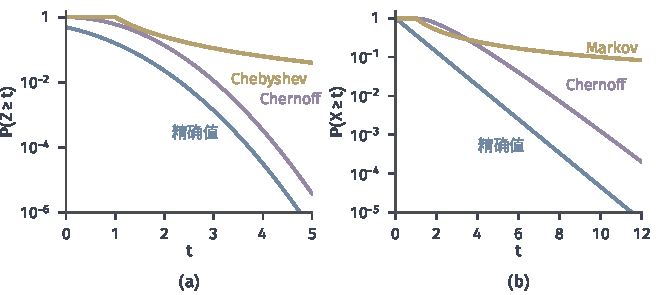
\includegraphics[width=112mm]{figures/07-probability/01-elementary-probability/matplotlib/tail-chernoff-compare/figure.pdf}
 \caption{精确右尾（蓝线）、指数矩上界（紫线）与矩上界（黄线），纵轴为对数刻度。(a)$Z\sim\mathcal{N}(0,1)$：$Q(t)$，$\mathrm{e}^{-t^2/2}$，Chebyshev界$\min\{1,1/t^2\}$。(b)$X\sim\operatorname{Exp}(1)$：$\mathrm{e}^{-t}$，$\min\{1,t\,\mathrm{e}^{1-t}\}$，Markov界$\min\{1,1/t\}$。}
 \label{fig:tail-chernoff-compare}
\end{BookInlineFigure}

\paragraph{指数矩有限与尾部指数衰减}
指数分布的例子说明，矩母函数在哪里有限，与尾部衰减得多快直接相关。图~\ref{fig:tail-mgf-domain}画出三个矩母函数：高斯分布的$\mathrm{e}^{\lambda^2/2}$处处有限；$\operatorname{Exp}(1)$的$1/(1-\lambda)$在$\lambda\to1$时趋于无穷；尺度为$1$的Laplace分布，按同样的积分得$1/(1-\lambda^2)$，只在$\lvert\lambda\rvert<1$时有限。

\begin{BookInlineFigure}
 \centering
 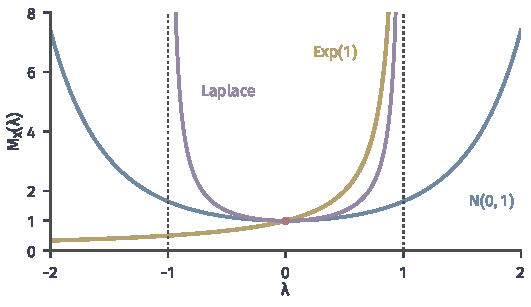
\includegraphics[width=90mm]{figures/07-probability/01-elementary-probability/matplotlib/tail-mgf-domain/figure.pdf}
 \caption{三个矩母函数。蓝线为$\mathcal{N}(0,1)$的$\mathrm{e}^{\lambda^2/2}$，黄线为$\operatorname{Exp}(1)$的$1/(1-\lambda)$（$\lambda<1$），紫线为尺度$1$的Laplace分布的$1/(1-\lambda^2)$（$\lvert\lambda\rvert<1$）。点线标出$\lambda=\pm1$，红点为所有矩母函数共有的$M_X(0)=1$。}
 \label{fig:tail-mgf-domain}
\end{BookInlineFigure}

一个方向已经由式~\eqref{eq:tail-chernoff-lambda}给出：只要某个$\lambda_0>0$使$M_X(\lambda_0)<\infty$，右尾就至少按$\mathrm{e}^{-\lambda_0t}$衰减。对非负、有密度的变量，反方向也成立。

\begin{theorem}[指数矩与尾部衰减]
\label{thm:tail-mgf-decay}
设$X\geq0$有密度，存在常数$C>0$、$c>0$，使$\mathbb{P}(X>s)\leq C\mathrm{e}^{-cs}$对一切$s\geq0$成立。则对$0\leq\lambda<c$，
\begin{equation}
 M_X(\lambda)\leq1+\frac{C\lambda}{c-\lambda}<\infty .
 \label{eq:tail-mgf-decay}
\end{equation}
\end{theorem}

\begin{proof}
在引理~\ref{lem:tail-integral}中取$g(s)=\mathrm{e}^{\lambda s}$，它连续可微且不减，$g(0)=1$，$g'(s)=\lambda\mathrm{e}^{\lambda s}$。于是
\[
 M_X(\lambda)=1+\int_0^{\infty}\lambda\mathrm{e}^{\lambda s}\,\mathbb{P}(X>s)\,\mathrm{d}s .
\]
代入尾部的假设，积分不超过
\[
 \int_0^{\infty}\lambda\mathrm{e}^{\lambda s}\,C\mathrm{e}^{-cs}\,\mathrm{d}s=C\lambda\int_0^{\infty}\mathrm{e}^{-(c-\lambda)s}\,\mathrm{d}s=\frac{C\lambda}{c-\lambda} .
\]
最后一步用到$c-\lambda>0$。
\end{proof}

对$\operatorname{Exp}(1)$，$C=c=1$，式~\eqref{eq:tail-mgf-decay}给出$1+\lambda/(1-\lambda)=1/(1-\lambda)$，与直接计算的结果相同。

\paragraph{重尾时没有指数矩}
尾部只按幂次衰减时，矩母函数在$\lambda>0$处全是无穷。对$\alpha=3$的Pareto分布，由幂级数的一项，$x\geq0$时$\mathrm{e}^{\lambda x}\geq(\lambda x)^3/6$，所以
\[
 M_X(\lambda)\geq\frac{\lambda^3}{6}\,\mathbb{E}[X^3]=+\infty,\qquad \lambda>0 .
\]
三阶矩已经无穷，指数矩更不可能有限。自由度有限的t分布、Cauchy分布也是如此。对这类分布，式~\eqref{eq:tail-chernoff}的下确界里没有任何可用的$\lambda$，只能退回到存在的那些矩。尾部按幂次衰减的分布通常称为\term{重尾分布}（heavy-tailed distribution），它们的矩上界在下一节单独检查。

\paragraph{左尾与双侧}
对左尾，把定理用于$-X$。对$\lambda>0$，事件$\{X\leq t\}$就是$\{-X\geq-t\}$，而$-X$在$\lambda$处的矩母函数是$M_X(-\lambda)$，于是
\begin{equation}
 \mathbb{P}(X\leq t)\leq\inf_{\lambda>0}\mathrm{e}^{\lambda t}M_X(-\lambda) .
 \label{eq:tail-chernoff-left}
\end{equation}
双侧事件按式~\eqref{eq:tail-two-sided}拆成两侧，各用一个界后相加。标准高斯分布关于$0$对称，两侧的界相同，得
\[
 \mathbb{P}(\lvert Z\rvert\geq t)\leq2\mathrm{e}^{-t^2/2},\qquad t>0 .
\]

\paragraph{本节的边界}
这里只用了单个随机变量的矩母函数。矩母函数还有两方面的用途：在一定条件下它决定分布本身，这类识别工具在第~\ref{chap:weak-convergence-of-distributions}章介绍；对许多独立量之和，它可以分解成各项矩母函数的乘积，于是式~\eqref{eq:tail-chernoff}给出样本平均偏离均值的指数界，可参考\BookChapterRef{chap:finite-sample-error-bounds}{卷八第4章“有限样本的误差上界”}。


\section{上界的评价}
\label{sec:tail-bound-comparison}

前面几节各自给出了一个界，每次都和精确值比了一比。现在把它们放在同一个变量、同一个阈值上，回答三个问题：每个界用了多少信息，在什么阈值上才有用，信息不全或矩不存在时还剩下什么。

\paragraph{同一事件上的排列}
对贯穿例子的事件$\{X\geq15\}$，表~\ref{tab:tail-bounds}列出各个界及其所需的信息。四阶、六阶矩界以$a=10$为中心，作用于包含$\{X\geq15\}$的双侧事件$\{\lvert X-10\rvert\geq5\}$；表的最后一行留到后面解释。

\begin{BookInlineTable}
 \centering
 \caption{$X\sim\operatorname{Bin}(20,1/2)$时$\mathbb{P}(X\geq15)$的精确值与各个上界。比值为上界除以精确值$0.0207$。}
 \label{tab:tail-bounds}
 \begin{tabular}{lllr}
  \toprule
  方法 & 所用信息 & 数值 & 比值\\
  \midrule
  精确值 & 完整质量表 & $0.0207$ & $1$\\
  Markov & $X\geq0$，$\mathbb{E}[X]=10$ & $0.667$ & $32$\\
  Chebyshev & $\mathbb{E}[X]$，$\operatorname{Var}(X)=5$ & $0.200$ & $9.7$\\
  四阶矩 & $m_4=72.5$ & $0.116$ & $5.6$\\
  六阶矩 & $m_6=1692.5$ & $0.108$ & $5.2$\\
  指数矩 & $M_X(\lambda)$，$\lambda>0$ & $0.0731$ & $3.5$\\
  最优原点矩 & $\mathbb{E}[X^k]$，$k\leq60$ & $0.0646$ & $3.1$\\
  \bottomrule
 \end{tabular}
\end{BookInlineTable}

图~\ref{fig:tail-bounds-bar}在对数刻度上画出同样的数。越往下，用到的信息越多，界越小，但即使是最好的界也比精确值大三倍。差距不会消失，因为每个界都是对一整类分布的保证：只要另一个分布与$X$有相同的已知数值而尾部更重，界就必须照顾它。

\begin{BookInlineFigure}
 \centering
 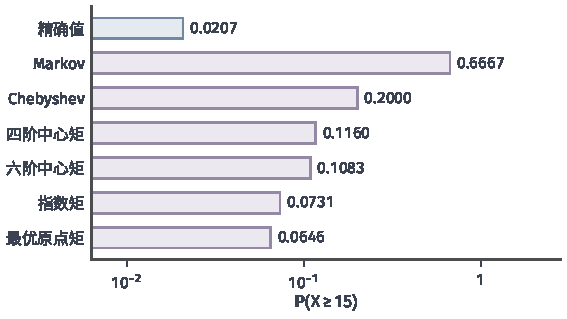
\includegraphics[width=96mm]{figures/07-probability/01-elementary-probability/matplotlib/tail-bounds-bar/figure.pdf}
 \caption{$X\sim\operatorname{Bin}(20,1/2)$时$\mathbb{P}(X\geq15)$的精确值（蓝）与各个上界（紫），横轴为对数刻度，数字为数值。四阶、六阶中心矩以$10$为中心；最优原点矩在$k=1,\dots,60$中取$\mathbb{E}[X^k]/15^k$的最小值，于$k=17$取到。}
 \label{fig:tail-bounds-bar}
\end{BookInlineFigure}

\paragraph{矩与指数矩的关系}
表中最后一行用的是原点矩$\mathbb{E}[X^k]$，对每个$k$由质量表求和，然后取$\mathbb{E}[X^k]/15^k$的最小值，在$k=17$处得到$0.0646$，竟比指数矩上界还小。这不是巧合：对非负变量，最好的矩上界从来不劣于指数矩上界。

\begin{theorem}[最优矩上界不劣于指数矩上界]
\label{thm:tail-moment-vs-chernoff}
设$Y\geq0$，$t>0$，$\lambda>0$且$M_Y(\lambda)<\infty$。则
\begin{equation}
 \inf_{k=0,1,2,\dots}\frac{\mathbb{E}[Y^k]}{t^k}\leq\mathrm{e}^{-\lambda t}M_Y(\lambda) .
 \label{eq:tail-moment-vs-chernoff}
\end{equation}
\end{theorem}

\begin{proof}
把$\mathrm{e}^{\lambda Y}$展成幂级数，各项$\lambda^kY^k/k!$都非负。非负项的级数可以与求和或积分交换次序，依据与引理~\ref{lem:tail-integral}证明中交换积分次序的依据相同，所以
\[
 M_Y(\lambda)=\sum_{k\geq0}\frac{\lambda^k\,\mathbb{E}[Y^k]}{k!} .
\]
两边乘$\mathrm{e}^{-\lambda t}$，并把每项写成“权重乘矩上界”：
\[
 \mathrm{e}^{-\lambda t}M_Y(\lambda)=\sum_{k\geq0}\Bigl(\mathrm{e}^{-\lambda t}\frac{(\lambda t)^k}{k!}\Bigr)\cdot\frac{\mathbb{E}[Y^k]}{t^k} .
\]
括号里的权重是参数为$\lambda t$的Poisson分布的质量，非负且和为$1$。记$b=\inf_k\mathbb{E}[Y^k]/t^k$，每个矩上界都不小于$b$，所以加权和不小于$b$：
\[
 \mathrm{e}^{-\lambda t}M_Y(\lambda)\geq b\sum_{k\geq0}\mathrm{e}^{-\lambda t}\frac{(\lambda t)^k}{k!}=b .
\]
这就是式~\eqref{eq:tail-moment-vs-chernoff}。
\end{proof}

证明说明了两者的关系：指数矩上界是各阶矩上界按Poisson权重的平均，平均值不会小于其中最小的一项。对右边取下确界后结论仍成立，所以式~\eqref{eq:tail-chernoff}的Chernoff界总不小于最优矩上界。定理要求$Y$非负，并且比较的是关于$0$的原点矩；对一般的$X$和单侧事件，可以取$Y=X$（当$X\geq0$时）或$Y=\lvert X-a\rvert$。

图~\ref{fig:tail-moment-vs-chernoff}在$Y=\lvert Z\rvert$、$Z\sim\mathcal{N}(0,1)$上验证这一点。$\lvert Z\rvert$的矩母函数为$2\mathrm{e}^{\lambda^2/2}\Phi(\lambda)$，其中$\Phi$是标准高斯分布函数，下确界需要数值计算。在$t=3$处，精确值、最优矩上界和指数矩上界依次为
\[
 0.0027,\qquad 0.0156,\qquad 0.0222 .
\]
两个界的差距不大，量级相同。

\begin{BookInlineFigure}
 \centering
 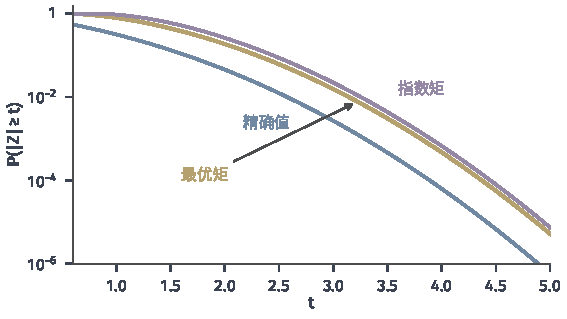
\includegraphics[width=96mm]{figures/07-probability/01-elementary-probability/matplotlib/tail-moment-vs-chernoff/figure.pdf}
 \caption{$Z\sim\mathcal{N}(0,1)$的$\mathbb{P}(\lvert Z\rvert\geq t)$（蓝线）、对实数阶$p>0$取最小的矩上界$\inf_p\mathbb{E}\lvert Z\rvert^p/t^p$（黄线）与$\lvert Z\rvert$的指数矩上界$\inf_{\lambda>0}\mathrm{e}^{-\lambda t}M_{\lvert Z\rvert}(\lambda)$（紫线），纵轴为对数刻度。}
 \label{fig:tail-moment-vs-chernoff}
\end{BookInlineFigure}

既然矩上界更紧，为什么还要指数矩？原因在计算。最优矩上界要求知道全部各阶矩，再对阶数搜索；指数矩把它们压缩成一个函数，常常有闭式，例如二项分布的$\bigl((1+\mathrm{e}^{\lambda})/2\bigr)^{20}$，只需一维最小化。对独立量之和，矩母函数还能分解成乘积，而高阶矩的展开会迅速变得繁琐。

\paragraph{反过来求试验次数}
界的差距在反问题中看得更清楚。掷$n$次均匀硬币，正面次数$X\sim\operatorname{Bin}(n,1/2)$，正面比例是$X/n$。要使比例偏离$1/2$至少$0.1$的概率不超过$0.05$，$n$至少要多大？

先用Chebyshev不等式。由第~\ref{chap:common-distributions}章，$\operatorname{Var}(X)=n/4$；由缩放规律，$\operatorname{Var}(X/n)=1/(4n)$。于是
\[
 \mathbb{P}\Bigl(\Bigl\lvert\frac{X}{n}-\frac12\Bigr\rvert\geq0.1\Bigr)\leq\frac{1/(4n)}{0.01}=\frac{25}{n} .
\]
要使右边不超过$0.05$，需要$n\geq500$。

再用指数矩上界。右侧事件是$\{X\geq0.6n\}$，在式~\eqref{eq:tail-binomial-chernoff-general}中取$p=1/2$，$a=0.6$，方括号里的数是
\[
 \Bigl(\frac{0.5}{0.6}\Bigr)^{0.6}\Bigl(\frac{0.5}{0.4}\Bigr)^{0.4}=\mathrm{e}^{-0.02014}\approx0.9801 .
\]
由对称性左侧事件$\{X\leq0.4n\}$有同样的界，两侧相加得$2\mathrm{e}^{-0.02014n}$。令它不超过$0.05$，解得$n\geq\ln40/0.02014\approx183.2$，即$n\geq184$。

最后用质量表直接计算。精确概率随$n$的变化并不单调，因为$0.6n$是否为整数会影响端点上的质量：$n=97$时约为$0.0417$，$n=100$时又升到$0.0569$。逐个计算可知，从$n=106$起精确概率都不超过$0.05$（数值检查到$n=500$）。三种方法给出的次数是$500$、$184$与$106$。上界越紧，为同一个保证付出的试验次数越少；精确计算最省，但要对每个$n$求和，而且只适用于确知的分布。

\paragraph{有效阈值}
每个界只在一段阈值上提供信息，在其余阈值上不小于$1$。Markov界在$t\leq\mathbb{E}[X]$时不小于$1$；Chebyshev界在$t\leq\sigma$时不小于$1$。指数矩上界在$t\leq\mathbb{E}[X]$时也给不出信息：由第~\ref{chap:random-variable-moments}章的Jensen不等式，$\mathrm{e}^{\lambda x}$是凸函数，所以
\[
 \mathrm{e}^{-\lambda t}M_X(\lambda)\geq\mathrm{e}^{-\lambda t}\mathrm{e}^{\lambda\mathbb{E}[X]}=\mathrm{e}^{\lambda(\mathbb{E}[X]-t)}\geq1,\qquad \lambda>0 .
\]
这符合直觉：阈值不在均值右边时，“越过阈值”并不是一个罕见事件。实际使用时把每个界与$1$取较小者，例如写成$\min\{1,\mathbb{E}[X]/t\}$；图中所有的界都已这样截断。

\paragraph{重尾模型}
对$\alpha=3$的Pareto分布，指数矩不存在，三阶及以上的矩也不存在，能用的只有$p<3$阶的矩。由$\mathbb{E}[X^p]=3/(3-p)$，原点矩上界是
\[
 \mathbb{P}(X\geq t)\leq\frac{3}{(3-p)\,t^{p}},\qquad 0<p<3 .
\]
$p$越接近$3$，$t^{-p}$衰减越快，但系数$3/(3-p)$越大。对给定的$t$，把对数$\ln3-\ln(3-p)-p\ln t$对$p$求导并令其为零：
\[
 \frac{1}{3-p}-\ln t=0,\qquad p^{*}=3-\frac{1}{\ln t} .
\]
当$t>\mathrm{e}^{1/3}\approx1.40$时$p^{*}\in(0,3)$，二阶导数$1/(3-p)^2>0$，这是最小点。

代回去，$3-p^{*}=1/\ln t$，$t^{-p^{*}}=t^{-3}\,t^{1/\ln t}=\mathrm{e}\,t^{-3}$，于是
\begin{equation}
 \inf_{0<p<3}\frac{3}{(3-p)\,t^{p}}=\frac{3\mathrm{e}\ln t}{t^{3}},\qquad t>\mathrm{e}^{1/3} .
 \label{eq:tail-pareto-best}
\end{equation}
精确值是$t^{-3}$，最好的原点矩上界多出一个因子$3\mathrm{e}\ln t$，随$t$缓慢增大。$t=10$时，界为$0.0188$，精确值为$0.001$。图~\ref{fig:tail-pareto-moments}在双对数坐标中画出这些曲线：每个固定阶数的界是一条斜率为$-p$的直线，红色虚线是它们的下包络。

\begin{BookInlineFigure}
 \centering
 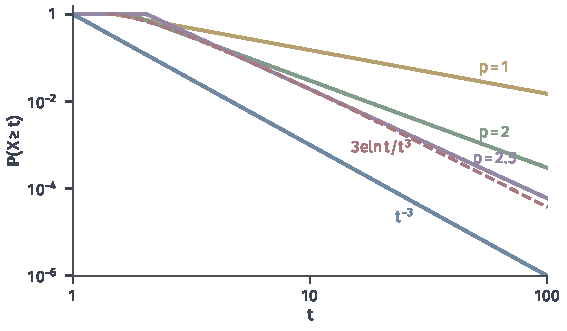
\includegraphics[width=96mm]{figures/07-probability/01-elementary-probability/matplotlib/tail-pareto-moments/figure.pdf}
 \caption{$\alpha=3$的Pareto分布，双对数坐标。蓝线为精确尾部$t^{-3}$，黄、绿、紫线为$p=1,2,2.5$的原点矩上界$\min\{1,3/((3-p)t^p)\}$，红色虚线为对$p\in(0,3)$取最小的包络$3\mathrm{e}\ln t/t^3$。}
 \label{fig:tail-pareto-moments}
\end{BookInlineFigure}

中心的选择同样重要。Pareto分布的均值为$3/2$，方差为$3-9/4=3/4$。对$t>3/2$，事件$\{X\geq t\}$包含在$\{\lvert X-3/2\rvert\geq t-3/2\}$中，Chebyshev不等式给出$\tfrac34/(t-\tfrac32)^2$。$t=10$时这是$0.0104$，反而比式~\eqref{eq:tail-pareto-best}的$0.0188$更好；$t=100$时它是$7.7\times10^{-5}$，又不如后者的$3.8\times10^{-5}$。以均值为中心去掉了原点处的偏移，在中等阈值上更有利；阈值很远时，阶数的作用占了上风。

更重的尾部会让可用的工具进一步减少。Cauchy分布连均值都没有，Markov不等式和Chebyshev不等式都不能用，只剩阶数$p<1$的绝对矩上界。这时尾概率本身也只按$1/t$衰减，任何依赖高阶矩的估计都无从谈起。

\paragraph{信息与代价}
图~\ref{fig:tail-information-ladder}把本章的界按所需信息排列。越往下，假设越强：均值有限弱于方差有限，方差有限弱于更高阶矩有限，而某个$\lambda>0$处指数矩有限蕴含一切阶矩有限。假设越强，界越紧，适用的分布越少。完整分布在最下面，它给出精确值，但需要的信息最多，计算也可能最难，例如高斯尾部$Q(t)$就要数值积分。

\begin{BookInlineFigure}
 \centering
 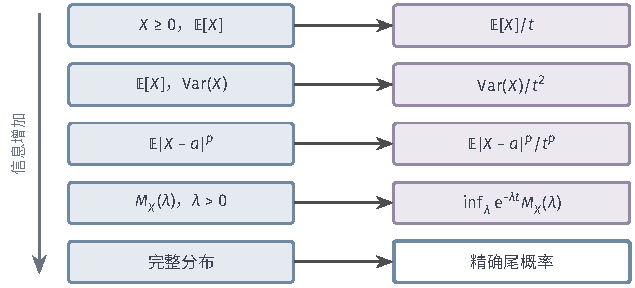
\includegraphics[width=108mm]{figures/07-probability/01-elementary-probability/tikz/tail-information-ladder/figure.pdf}
 \caption{所用信息（左）与得到的尾部结论（右）。前两行分别控制$\mathbb{P}(X\geq t)$与$\mathbb{P}(\lvert X-\mathbb{E}[X]\rvert\geq t)$，第三行控制$\mathbb{P}(\lvert X-a\rvert\geq t)$，第四行控制$\mathbb{P}(X\geq t)$。自上而下大致按所需的矩条件由弱到强排列，紫色为上界，白色为精确值。}
 \label{fig:tail-information-ladder}
\end{BookInlineFigure}

计算成本按相反方向排列。Markov界和Chebyshev界只要一两个数，一次除法；矩上界要计算一个积分或求和；指数矩上界要先得到矩母函数，再做一维最小化，可以求导，也可以数值搜索；精确值要对整个尾部求和或积分。实际选择时先问手上有什么信息，再问需要多紧的保证。

\paragraph{保证与估计}
最后要分清三种数。精确尾概率是具体分布的性质。Markov界和Chebyshev界在各自的信息下是最好的保证，第~\ref{sec:tail-markov}节和第~\ref{sec:tail-chebyshev}节的极端分布达到了它们，所以不能指望仅凭这些信息改进。矩上界与指数矩上界则依赖额外的假设：高阶矩或指数矩存在，并且已知其数值。额外的假设换来了更紧的界，也缩小了适用范围；假设一旦不成立，例如遇到重尾模型，就要退回到弱的界。


\section{本章小结}
\label{sec:tail-summary}

本章从尾事件出发。右尾$\{X\geq t\}$、左尾$\{X\leq t\}$与双侧事件$\{\lvert X-a\rvert\geq t\}$的概率都可以由分布函数算出，但端点要分清：含原子时$\mathbb{P}(X\geq t)=1-F_X(t^-)$，比$1-F_X(t)$多出$\mathbb{P}(X=t)$；双侧事件拆成两个不相交的单侧事件，不对称的分布要两侧分别计算。对非负变量，期望是生存函数下的面积，各阶矩也由尾部决定，尾部衰减得慢，高阶矩就不存在。

只知道少量数值特征时，所有的界都来自同一个想法：用一个非负不减的函数从上方压住尾事件的示性函数，再取期望。压法不同，用到的信息就不同。非负变量的均值给出Markov不等式$\mathbb{E}[X]/t$；方差给出Chebyshev不等式$\sigma^2/t^2$；$p$阶绝对矩给出按$t^{-p}$衰减的界；指数矩给出Chernoff界$\inf_{\lambda>0}\mathrm{e}^{-\lambda t}M_X(\lambda)$，在高斯和二项模型上它能抓住尾部的指数衰减。

这些界要与真实概率分开理解。Markov界和Chebyshev界在各自的信息下不能改进，两点和三点极端分布达到它们，所以与具体模型的差距来自信息不足，而不是论证粗糙。更高阶的矩和指数矩是额外的假设：它们给出更紧的界，但要求更强的存在条件，阶数越高也不保证对每个阈值越好。对非负变量，最优的矩上界不劣于指数矩上界，指数矩的优势在于便于计算。重尾模型把这些限制暴露出来：Pareto分布只有低阶矩，Cauchy分布连均值都没有，可用的界随之变弱；界大于$1$时直接与平凡界$1$取较小者。

后面的章节会反复回到这些不等式。判断一列随机变量是否越来越集中在某个值附近，说明许多次独立试验的平均值稳定在均值附近，以及保证用随机样本估计积分时误差不太大，出发点都是Markov和Chebyshev不等式；把指数矩用于许多独立量之和，则得到随试验次数指数缩小的误差保证。

